\section{Theory}
\subsection{Blood}
\label{bloodtheory}
The heart pumps blood through a great system of arteries and veins in order to supply oxygen to the living tissue and take away carbon dioxide. Next to that, blood is also responsible for collecting food from the intestines and neutralizing foreign biological agents which enter the system, among others \cite{rheologyofblood}. Blood is not a simple liquid but a suspension of formed elements including red cells, white cells and platelets in a saline solution of three major types of protein. 

The red blood cells (RBCs) are in the blood to transport the oxygen and carbon dioxide and is most present in the blood. Red blood cells are most present in blood, averaging 40-45 volume\% of the blood. The volume\% of RBCs is also called the hematocrit. When there is a low shear stress on blood, it will form rouleaux \cite{merill}. Rouleaux is a cylindrical structure formed by red blood cells joined face-to-face, in combination with fibrinogen. This structure and the red blood cells themselves are shown in \autoref{RBCs}.
\begin{figure}[b]
\centering
	\begin{subfigure}[b]{0.4 \textwidth}
	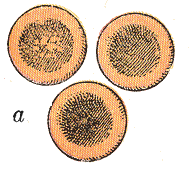
\includegraphics[scale = 0.75]{gray-a.png}
	\caption{Red blood cells front view \cite{GRAY}}
	\label{rbcfront}
	\end{subfigure}
	%\hfill
	\begin{subfigure}[b]{0.55 \textwidth}
	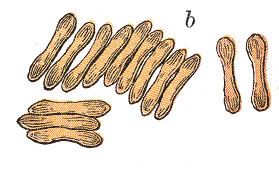
\includegraphics[scale = 0.75]{gray-b.png}
	\caption{Rouleaux formed and a side view of red blood cells \cite{GRAY}}
	\label{rouleaux}
	\end{subfigure}
\caption{Front and side view of red blood cells in a rouleaux}
\label{RBCs}
\end{figure}
The effect of the properties of blood (i.e. containing red blood cells and other components) on the flow of blood will be discussed in this paper. In \autoref{viscositysection} will be discussed what the effects are on the fluid properties of blood, while in MODELS FOR it will be discussed how the fluid flow can be simulated. These simulations will lead to the comparison of different viscosity models for blood rheology and how those affect flow and wall shear stress in arteries. 
\subsection{Viscosity}
\label{viscositysection}
\subsubsection{Viscosity in general}
Laminar flow can be described as a flow that is neatly ``layered'', meaning that there are infinitesimal small layers in the flow direction which have the same speed. These layers move at different speeds from each other but have a contact surface, and through this speed difference there is a friction. This friction force per surface area is called shear stress and is denoted as $\tau_{yx}$, which means that the shear stress is acting in the x direction on a surface normal to the y plane. 

A measure of the deformation of the fluid caused by this shear stress can be described by the strain rate (the amount of strain per second), which can be written as (in a 1 dimensional flow in the $x-$direction)
\begin{equation}
\dot{\gamma} = \frac{du_{x}}{dt}
\end{equation}
in which $\dot{\gamma}$ is the strain rate and $u$ is the speed in the fluid flow direction \cite{nonnewtonianflow}. If a fluid's shear stress is linearly proportional to the shear rate applied, it is said to be a Newtonian fluid and can be described as
\begin{equation}
\tau_{yx}= -\mu \frac{du_{x}}{dy}
\end{equation}
where $\mu$ is the viscosity. This equation is negative because a bigger velocity gradient is a bigger friction, thus exerting a force in the \emph{opposite} direction\cite{FT}. Water and air are common Newtonian fluids.

In Newtonian fluids, the viscosity is a material property dependent on temperature and pressure for different fluid systems. A high viscosity means that there is a lot of resistance to a velocity gradient and makes a very thick fluid, while a low viscosity makes a very fluent fluid.

In Newtonian fluids, the relatively small and round particles are only impeded in movement by each other. This is why most fluids are not Newtonian! Blood is not Newtonian because blood is not a uniform fluid (see \autoref{bloodtheory}).
\subsubsection{Non-Newtonian viscosity}
When the fluid's viscosity is not only dependent on the temperature and the density but also on the shear rate, that fluid is called non-Newtonian. Most fluids start at a zero shear rate `first Newtonian' value for the viscosity called $\mu_{0}$ to a `second-Newtonian'value $\mu_{2}$ at very high shear rates \cite{nonnewtsimulation}. When this is the case, the fluid is said to be shear-thinning, or pseudoplastic. The opposite can happen as well, when the apparant viscosity (the viscosity at a certain shear stress) starts lower and ends higher. Lastly there's Bingham plastics, who only start flowing when there is a certain shear stress applied. A well-known example of this is toothpaste \cite{FT}. In \autoref{viscosityplaatje} there is an overview of different types of fluid and their viscosity behavior plotted against shear stress.
\begin{figure}[hb]
\centering
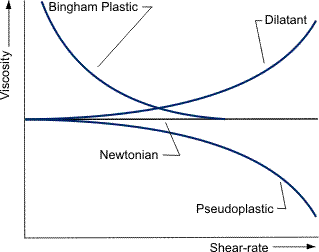
\includegraphics{viscosityshearstress.png}
\caption{The viscosity of a fluid plotted against the shear stress \cite{viscositypicture}}
\label{viscosityplaatje}
\end{figure}
Blood has been tested to be a shear-thinning fluid \cite{bloodthinning}. 
 
The viscosity of blood has been generally accepted as temperature \emph{independent} because it has very little effect on the viscosity nor on the yield stress\cite{rheologyofblood}.


\subsection{CFD}
Computational Fluid Dynamics (or CFD) is based on the Newtonian principles of
\begin{itemize}
\item The conservation of mass
\item The conservation of momentum
\item The conservation of energy
\end{itemize}
The conservation of mass is also known as the equation of continuity. In words this equation describes that there is only accumulation of mass due to mass coming in or leaving the control volume. In formula form this would be
\begin{equation}
\label{continuity1}
\frac{\partial \rho}{\partial t} = -\left(\nabla \cdot \rho{\bf u}\right)
\end{equation}
where $\rho$ is the density, ${\bf u}$ is the velocity vector and $\left(\nabla \cdot \rho{\bf u}\right)$ is the ``divergence'' of $\rho{\bf u}$ (the massflux). The divergence tells us about the net rate of massflux leaving the control volume, hence the - sign. For incompressible flows (such as blood\cite{merill}), the density is constant, whch transforms \autoref{continuity1} into
\begin{equation}
\left(\nabla\cdot{\bf u}\right) = 0
\end{equation}
The conservation of momentum is also known as the equation of motion. In words this equation describes that change in momentum of the control volume is a direct cause of the difference in momentum entering and leaving the system \emph{plus} the sum of the force acting of the control volume. In formula form this would be
\begin{equation}
\label{NVST}
\frac{\partial}{\partial t}\rho{\bf u} = -\left[\nabla \cdot \rho{\bf uu}\right] -\nabla p -\left[\nabla \cdot {\bm \tau} \right] + {\bf f}
\end{equation}
where $p$ is the pressure, $\bm \tau$ is the shear stress tensor(discussed in \autoref{viscositysection}), and $\bf f$ is the sum of all forces on the element. This is also called the Navier-Stokes equation and governs the movement of incompressible fluids. It should be noted that $\left[\nabla \cdot \rho{\bf uu}\right]$ and $\left[\nabla \cdot {\bm\tau} \right]$ are not divergences because $\bm \tau$ and $\bf uu$ are tensors and not vectors. For incompressible fluids, \autoref{NVST} can be simplified to 
\begin{equation}
\label{incNVST}
\rho\left(\frac{\partial{\bf u}}{\partial t} + {\bf u} \cdot \nabla{\bf u}\right) = -\nabla p - \left[\nabla \cdot{\bm \tau}\right] + {\bf f}
\end{equation} 
And $\bm \tau$ is defined as
\begin{equation}
\bm \tau = \begin{bmatrix}
			\tau_{xx} & \tau_{xy} & \tau_{xz} \\
			\tau_{yx} & \tau_{yy} & \tau_{yz} \\
			\tau_{zx} & \tau_{zy} & \tau_{zz} 
			\end{bmatrix}
\end{equation}
More information on the continuity equation and the Navier-Stokes can be found in \cite{TP}.

The conservation of Energy only plays a role in temperature dependent systems, while we assume for blood to be near constant temperatures in the body. Because we say that density is constant and $\mu$ to be only dependent on shear stress, we will neglect temperature in this study. 
